When simulating quantum circuits on a \Simulator, it is generally unnecessary to consider whether the quantum circuit can actually be executed on a quantum chip. Our focus lies solely on investigating the feasibility of the algorithm. However, when accounting for real quantum chips, the set of quantum gates executable on the chip is finite. Moreover, due to the existence of quantum noise, it is desirable to minimize the depth of the quantum circuit. This necessitates the compilation and optimization of the quantum circuit. In this section, we will elucidate how \MindQuantum\ performs the compilation and optimization of quantum circuit.

Here, we use DAG (Directed Acyclic Graph) as a tool to compile quantum circuit. As shown in Fig~\ref{fig:compiler}, a quantum circuit is converted to a DAG. Based on the DAG we can apply built-in compilation rules, such as \BasicDecompose, \FullyNeighborCanceler and \GateReplacer, in \MindQuantum\ to finish quantum compilation and optimization. Furthermore, we have two robust managers in place for organizing these compilation rules, which are \SequentialCompiler and \KroneckerSeqCompiler. The rules in \SequentialCompiler will perform one by one in single time, but the rules in \KroneckerSeqCompiler will be executed until they can not compile anymore.

\begin{figure}
    \centering
    \begin{subfigure}{0.25\textwidth}
        \centering
        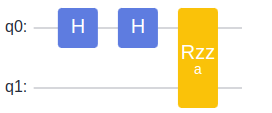
\includegraphics[width=\textwidth]{images/8_1_ori_circ.png}
        \caption{The original quantum circuit.}
        \label{fig:compiler_a}
    \end{subfigure}
    \begin{subfigure}{0.3\textwidth}
        \centering
        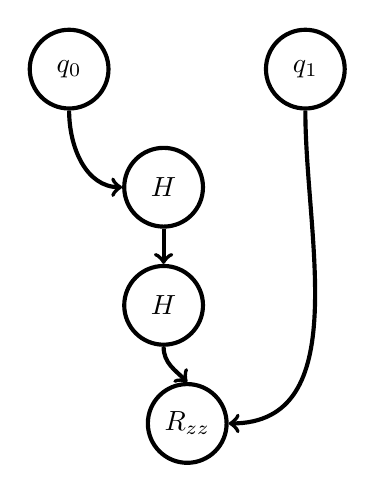
\begin{tikzpicture}[
                transparent/.style={circle, draw=black, fill=none, font=\sffamily, text centered, line width=1.5pt, minimum size=1cm}
            ]
            \node (q0) at (0, 0) [transparent] {$q_0$};
            \node (q1) at (3, 0) [transparent] {$q_1$};
            \node (H1) at (1.2, -1.5) [transparent] {$H$};
            \node (H2) at (1.2, -3) [transparent] {$H$};
            \node (Rzz) at (1.5, -4.5) [transparent] {$R_\text{zz}$};
            \draw [->, line width=1.5pt] (q0.south) to[out=270, in=180] (H1.west);
            \draw [->, line width=1.5pt] (H1.south) to[out=270, in=90] (H2.north);
            \draw [->, line width=1.5pt] (H2.south) to[out=270, in=135] (Rzz.north);
            \draw [->, line width=1.5pt] (q1.south) to[out=270, in=0] (Rzz.east);
        \end{tikzpicture}
        \caption{The DAG representation of quantum circuit.}
    \end{subfigure}
    \begin{subfigure}{0.45\textwidth}
        \centering
        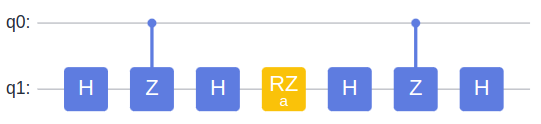
\includegraphics[width=\textwidth]{images/8_1_compiled_circ.png}
        \caption{The circuit after compilation and optimization.}
        \label{fig:compiler_c}
    \end{subfigure}
    \caption{Converting a quantum circuit to DAG and compile it to with given compile rules.}
    \label{fig:compiler}
\end{figure}

As an example, we will use different rules to compile and optimize the circuit in Fig~\ref{fig:compiler_a}. First we build a \KroneckerSeqCompiler with \BasicDecompose and \FullyNeighborCanceler, so that we can decompose the $R_\text{zz}$ gate into basic quantum gate and canceled the two Hadamard gates. Next, we will replace the CNOT gate to CZ gate, assuming that the chip can only execute CZ gate.
\begin{lstlisting}
from mindquantum.core.circuit import Circuit
from mindquantum.algorithm.compiler import *

circ = Circuit().h(0).h(0).rzz('a', [0, 1])

compiler = SequentialCompiler([
    KroneckerSeqCompiler([
        BasicDecompose(),
        FullyNeighborCanceler()
    ]),
    CXToCZ()
])

new_circ = compile_circuit(compiler, circ)
\end{lstlisting}
